\documentclass[11pt]{article}

\usepackage[margin=1in, paperwidth=8.5in, paperheight=11in]{geometry}
\usepackage{amsmath}
\usepackage[document]{ragged2e}
\usepackage{graphicx}
\usepackage{listings}
\usepackage{color}
\usepackage{interval}

\definecolor{dkgreen}{rgb}{0,0.6,0}
\definecolor{gray}{rgb}{0.5,0.5,0.5}
\definecolor{mauve}{rgb}{0.58,0,0.82}

\lstset{frame=tb,
  language=Python,
  aboveskip=3mm,
  belowskip=3mm,
  showstringspaces=false,
  columns=flexible,
  basicstyle={\small\ttfamily},
  numbers=none,
  numberstyle=\tiny\color{gray},
  keywordstyle=\color{blue},
  commentstyle=\color{dkgreen},
  stringstyle=\color{mauve},
  breaklines=true,
  breakatwhitespace=true,
  tabsize=3
}


\begin{document}


\title{\textbf{Generalized linear model: Bioassay with Metropolis}}
\maketitle


To implement the algorithm, I have used \textbf{10 chains}.

Every chain has \textbf{4000 samples}.

The \textbf{warm-up/burn-in length is 1000}.

The starting points for the chains are:
\\~\\
\begin{center}

\begin{tabular}{c|c|c}
$ n $ & $ \alpha $ & $ \beta $ \\ \hline
1 & -1 & 13 \\
2 & 0 & 0 \\ 
3 & -2 & 28 \\
4 & -3 & 13 \\
5 & -4 & -5 \\
6 & 3 & -4 \\ 
7 & -1 & 3 \\ 
8 & -1 & 7 \\
9 & 0 & 22 \\
10 & 4 & 4
\end{tabular}

\end{center}


I used the following \textbf{proposal distribution}:

\begin{lstlisting}
def proposal(theta_prev, cov):
    jump = stats.multivariate_normal(theta_prev, cov)
    theta_sample = jump.rvs(1)
    return np.array(theta_sample)
\end{lstlisting}

It is calculated using the multivariate normal distribution of the previous $ \theta $ and the covariance matrix \mbox{divided} by 10.

The ratio of the densities is calculated with the following formula:
$$ r = \frac{p(\theta^* | y)}{p(\theta^{t-1} | y)} $$
\\~\\

The $ \mathbf{\hat{R}} $ for $ \alpha $ and $ \beta $ are:
\\~\\
$ \mathbf{ \left[ 1.00715495, 1.01302307 \right] } $
\\~\\
and they are calculated using the \textbf{psrf} function, which was provided for us.

Alternatively, we can use the following formula to calculate the $ \hat{R} $:
$$ \hat{R} = \frac{\hat{var} + (\Psi | y)}{W} $$
\\~\\
If the \textbf{PSRF} values are not close to 1, then that means that the chain has not converged yet and that we should proceed with further simulations.
\\
In my case the values are close to 1, which mean that the chain \textbf{has converged}.


\begin{center}
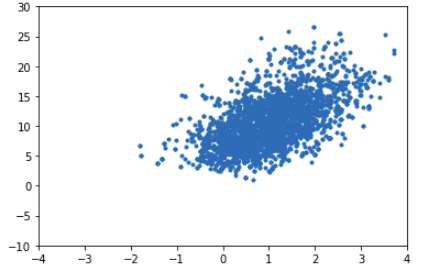
\includegraphics[width=10cm, height=5cm]{scatter.png}
\\
\textbf{Figure 1:} 10 Chains with 39000 samples in total (4000 * 10 - warm-up)
\end{center}


\newpage
\begin{align}
\textbf{SOURCE CODE}
\end{align}

\begin{lstlisting}

import matplotlib.pyplot as plt
from scipy import stats
import numpy as np
import random


def psrf(X, return_extra=False):
    # Handle input
    X = np.asarray(X)
    if X.ndim == 2:
        X = X[np.newaxis]
    # Split chains
    M = X.shape[0]*2
    N = X.shape[1]//2
    D = X.shape[2]
    if X.shape[1]%2 == 0:
        X = X.reshape((M,N,D))
    else:
        # Discard the middle samples (data copied)
        X_in = X
        X = np.empty((M,N,D), dtype=X_in.dtype)
        np.copyto(X[:X_in.shape[0]], X_in[:,:N])
        np.copyto(X[X_in.shape[0]:], X_in[:,-N:])
    
    if N <= 2:
        raise ValueError("Too few samples")
    
    # Means of the variances
    W = np.mean(np.var(X, axis=1, ddof=1), axis=0)
    # Variances of the means
    B = np.var(np.mean(X, axis=1), axis=0, ddof=1)
    
    # Calculate reduction factors
    Vh = W*(N-1)/N + B
    B *= N
    R = np.sqrt(Vh/W)
    
    if not return_extra:
        return R
    
    else:
        # Autocorrelation
        temp_1 = np.empty_like(X)
        rho = np.ones((N,D))
        for t in xrange(1,N):
            tempslice = temp_1[:,:-t]
            np.subtract(X[:,:-t], X[:,t:], out=tempslice)
            np.square(tempslice, out=tempslice)
            np.sum(tempslice, axis=(0,1), out=rho[t])
            rho[t] /= 2*M*(N-t)*Vh
        np.subtract(1, rho[1:], out=rho[1:])
        
        # Effective sample size
        mid = N//2
        cp = np.sum(np.reshape(rho[:2*mid], (mid,2,D)), axis=1)
        # The following could be Cythonised
        ci = np.argmax(cp<0, axis=0)
        no_init_pos = np.nonzero(np.all(cp>=0, axis=0))[0]
        if len(no_init_pos) > 0:
            print (
                "Initial positive could not be found for variable(s) {}, "
                "maxlag value used.".format(no_init_pos+1)
            )
            ci[no_init_pos] = mid
        cp *= np.arange(mid)[:,np.newaxis] < ci
        tau = -1 + 2*np.sum(cp, axis=0)
        neff = M*N/tau
        
        return R, neff, Vh, W, B, tau
        
        
def bioassaylp(a, b, x, y, n):
    a = np.expand_dims(a, axis=-1)
    b = np.expand_dims(b, axis=-1)
    # these help using chain rule in derivation
    t = a + b*x
    et = np.exp(t)
    z = et/(1.+et)
    for i in range(len(z)):
        if z[i] < 1e-12:
            z[i] = 1e-12
        if z[i] == 1:
            z[i] -= 1e-12
            
    # negative log posterior (error function to be minimized)
    lp = np.sum(y*np.log(z)+ (n-y)*np.log(1.0-z), axis=-1)
    return lp
    
    
n = np.array([5, 5, 5, 5])
x = np.array([-0.86, -0.30, -0.05, 0.73])
y = np.array([0, 1, 3, 5])
corr = 0.5
sigma_a = 2
sigma_b = 10
mu_a = 0
mu_b = 10
p = 0.5

mean = np.array([mu_a,mu_b])
covariance = np.array([[sigma_a**2,p*sigma_a*sigma_b],[p*sigma_a*sigma_b,sigma_b**2]])


def proposal(theta_prev, cov):
    jump = stats.multivariate_normal(theta_prev, cov)
    theta_sample = jump.rvs(1)
    return np.array(theta_sample)


def next_theta(theta_prev, cov): 
    theta_new = proposal(theta_prev, cov)
    
    likelihood_new = bioassaylp(theta_new[0], theta_new[1], x, y, n)
    likelihood_prev = bioassaylp(theta_prev[0], theta_prev[1], x, y, n)

    prior_multivariate_normal = stats.multivariate_normal(mean, covariance)
    prior_new = prior_multivariate_normal.pdf(theta_new)
    prior_prev = prior_multivariate_normal.pdf(theta_prev)

    post_new = np.exp(likelihood_new) * prior_new
    post_prev = np.exp(likelihood_prev) * prior_prev
    ratio = post_new / post_prev

    
    # check if theta_new gets accepted    
    if ratio >= 1:
        return theta_new
    else:    
        uniform = stats.uniform(0,1)
        random_sample = uniform.rvs(1)[0]
    if random_sample < ratio:
        return theta_new
    else:
        return theta_prev
    


def chaining(sample_len, number_of_chains, warm_up):
    chains = []
    for i in range(number_of_chains):
        random_point = [random.randint(-4, 4), random.randint(-10, 30)]
        print('starting points', random_point)
        random_point = [random_point]
        for j in range(sample_len):
            chain = next_theta(random_point[-1], covariance/10)
            random_point.append(chain)

    chains.append(random_point[warm_up:])
    return chains



chains = chaining(sample_len=4000, number_of_chains=10, warm_up=1000)
for chain in chains:
    plt.plot(
        np.array(chain)[:, 0],
        np.array(chain)[:, 1],
        marker = '.',
        linewidth = 0,
    )


plt.xlim(-4, 4)
plt.ylim(-10, 30)
plt.show()
print('PSRF value is: {0}'.format(psrf(chains)))

\end{lstlisting}

\end{document}




